%
% File acl-hlt2011.tex
%
% Contact: gdzhou@suda.edu.cn
%%
%% Based on the style files for ACL2008 by Joakim Nivre and Noah Smith
%% and that of ACL2010 by Jing-Shin Chang and Philipp Koehn


\documentclass[11pt]{article}
\usepackage{acl-hlt2011}
\usepackage{times}
\usepackage{latexsym}
\usepackage{amsmath}
\usepackage{multirow}
\usepackage{url}
\usepackage{graphicx}
\DeclareMathOperator*{\argmax}{arg\,max}
\setlength\titlebox{6.5cm}    % Expanding the titlebox

\title{What's up, Wikipedia? What is popular on Wikipedia and why.}

\author{Byung Gyu Ahn, Chris Callison-Burch, Benjamin Van Durme \\
  Center for Language and Speech Processing \\
  Johns Hopkins University \\
  Baltimore, Maryland \\
  {\tt \{bahn, ccb, vandurme\}@cs.jhu.edu} \\}

\date{}

\begin{document}
\maketitle
\begin{abstract}
The popularity that social networks such as Twitter and Facebook have recently gained calls more research into the use of metadata that they generate. In this paper, we make use of the page view counts of Wikipedia articles to predict topics gaining in popularity and explain why these topics are gaining users' attention. Our proposed approach clusters related topics to distinguish the main topics of on-going events from secondary related topics and explains the relationship between them. We explain why this is an interesting problem and compare approaches using the link structure of Wikipedia articles and the bag of words model of them to process each step of the process. By combining each step that performs reasonably as well as human annotators, the methods put forth here make a nice summary of what people in the real world are really insterested in.

For sets of articles that show a sharp increase i page view on the same date, we do the following:
(1) cluster articles into subsets that correspond to the same current event, (2) select sentences from the articles that describe why the event is popular.
We evaluate against manually clustered articles and hand selected sentences.
We show the value of bag-of-words topic models, link structure, named entity and time expression recognition.
The result shows promise for explaining what's currently popular on Wiipedia and for creating a timeline of past newsworthy events.

\end{abstract}

\section{Introduction}

Recently, social media such as Twitter and Facebook gained attention from researchers.
By looking at the topics recently prevailing in a lot of Twitter data at the same time, one may know the recent popular topics.

%Wikipedia has some relative advantage over Twitter as a source of topics, in that (1) it has a full description about the topic, (2) it has inter-article links that imply the relations between articles, and (3) the page view statistics are open to the public.

%The page view statistics are publicized in one of the wikipedians' website. Hour-by-hour statistics of size of 50-80Mbytes, each gzipped. The unzipeed file contains the project name, the article title, the page view counts, and the page size per line.

\cite{LDC:04} describes the definition of topics and events used in the TDT dataset. 

%* System overview describing each module, and including a diagram of how they connect (1.5 pages)
 %- include description of hour-by-hour wikipedia page view stats
   %+ show example graphs that highlight trending topics

%We first discuss previous work related to our work (\S2), then discuss our experimental design (\S3), and move on to show our experimental result (\S4). We then discuss our future work (\S5).

%There is an open-source software called Trending Topics (\url{http://www.trendingtopics.org/}) that shows the recent popular topics extracted from Wikipedia. We employed the same algorithm, which sorts the topics by the difference between the sum of the page counts of the recent 15 days and the sume of the page counts of the previous 15 days. Then, we picked the 100 topics of the highest differences.

In this paper we analyze a novel data set: we have collected the hourly page view statistics for every Wikipedia page in every language for an X year period. We show how these page view statistics--along with a whole host of other features like inter-page links, edit histories, mentions in contemporaneous news stories--can be used to identify and explain popular trends, including political elections, natural disasters, sports championships, popular films and music, and other current events.

Our approach is to select a set of articles whose daily page views increase by XXX\% or more above their average from the previous two week period. Rather than simply selecting the most popular articles for a given day, this selects articles whose popularity is rapidly increasing. These popularity spikes are presumably due to some external current event in the real world. On any given day, there are many articles whose popularity is spiking.

In this paper we attempt to cluster 100 such articles from each of 5 randomly selected days in 2009, such that the clusters coherently correspond to current eents.

Mention Wikipedia current events, and why we did not use them as our gold standard. They are boring events that do not generate much traffic, and that link to pages that are too general like ``United States'' or ``Israel''. We view this work as an automatic mechanism that could potentially supplant the hand-curated method of selecting current events that is currently done by Wikipedia editors.

For instance, we would attempt to cluster the articles in Figure~\ref{fig:} into 3 clusters, \{ Barack Obama, Joe Biden, White House, Inauguration \} which corresponds to the inauguration of Barack Obama, \{ US Airways Flight 1549, Chesley Sullenburger, Hudson River \} which corresponds to the successful ditching of an airplane into the Hudson river without loss of life, and \{ Superbowl, Arizona Cardinals \} which describes the then upcoming Superbowl XLIII.

We further try to explain the clusters by selecting sentences from the revision of the Wikipedia articles on that date. For the first cluster, a good selection might be "the inauguration of Barack Obama as the 44th president of the United States took place on Jan 20, 2009". [take the first sentence from Chesley's article] [Superbowl XLIII] will feature the... (the second setence, which makes clear the relationship with Arizona Cardinals.

To generate the clusters we can make use of the text of the articles on that date, versions of the articles from previous dates, the link structure and category info from Wikipedia, and potentially external info like newspaper articles published before the date.

To select sentences we may want to make use of NLP technologies such as coref resolution, named entity and date taggers, and dependency parsers to identify subjects of sentences.

\section{Motivation}

What are interesting topics? This could be an aesthetic question, but, in Wikipedia, gaining popularity usually means a big inflow of users looking up an article of a specific topic. More often than not, a popular on-going event accompanies many topics, or Wikipedia articles, collecting sudden increases in page view counts (Figure~\ref{fig:topics-for-an-event}). The TrendingTopics\footnote{Should we put a space between Trending and Topics?} algorithm (\S\ref{sec:related-work}) finds a big increase in page view counts and make a list of the articles with the highest increase. 

The wikipedia has a section called current events, in which the recently occurred events are listed manually by Wikipedians\footnote{Should Wikipedians be capitalized or not?}. Some of the most charateristic instances from the topics and the events are shown in Table~\ref{tab:topics-events-comparison}. We evaluated the precision and recall score of the TrendingTopics topics against the Wikepedian Current Events (Table~\ref{tab:topics-events-evaluation}. Their precision and recall scores are extremely low. Probably, wikipedians are more interested in political and scientific topics, and the page view statistics tend to be more dramatic for the societal and cultural events--recent deaths of famous people, recent release of movies and music albums.

Due to the discrepancy between the Wikipedian Current Events and the topics based on page views, it was not realistic to predict from the page view counts the topics that would overlap the Current Events. We set the topics extracted by the TrendingTopics algorithm as the baseline data.

\begin{figure*}
\centering
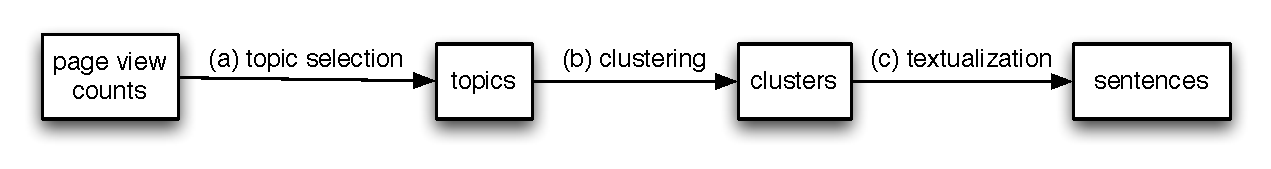
\includegraphics[width=0.8\textwidth]{figures/acl11-process.pdf}
\caption{Process diagram. (a) Topic selection. (b) Clustering. (c) Textualization.}
\label{fig:process}
\end{figure*}

%Figure~\ref{fig:process} outlines the subprocesses discussed in this paper. The first phase, {\it topic selection} is the step that 

%\section{Topic selection}

%\paragraph {Design}
%\begin{figure}
%\begin{picture}(200,100)
%\end{picture}
%\caption{A sparkline graph that shows page views of related topics of an event.}
%\label{fig:topics-for-an-event}
%\end{figure}

%\begin{table}
%\begin{tabular}{|c|}
%\hline
%TrendingTopics algorithm \\
%\hline
%Recent deaths \\
%Recent album releases \\
%Recent movie releases \\
%Recent news \\
%\hline
%Current Events\\
%\hline
%Political events \\
%Social events \\
%\hline
%\end{tabular}
%\caption{Examples of the topics collected by the TrendingTopics algorithm and the Current Events by Wikipedians.}
%\label{tab:topics-events-comparison}
%\end{table}

%\begin{table}
%\begin{picture}(200,100)
%\end{picture}
%\caption{Evaluation of the TrendingTopics topics against the Current Events}
%\label{tab:topics-events-evaluation}
%\end{table}

Our system is described as follows. First, the most popular pages, or topics, are collected per each day. Second, clusters are identified by clustering related topics. Third, the main cluster of each cluster is identified. Lastly, the sentence that best describes the cluster are extracted for each cluster.

\section{Clustering}
\label{ssec:clustering}

\begin{table}
\begin{tabular}{|c|}
\hline
Barack\_Obama \\
Inaugural\dots \\
\dots \\
The names of past presidents...\\
\dots \\
Hudson\_River... \\
\hline
\end{tabular}
\caption{Topics for January 27th, 2009.}
\label{tab:topics-example}
\end{table}

Once extracted, the topics include individual articles that can be divided into some categories (see Table~\ref{tab:topics-example}). The categories, however, are somewhat random and highly related to on-going events. In many cases, there are ``central'' topics that are directly relevant to an on-going event, and there are ``peripheral'' topics that are weakly related to the same events. In Figure~\ref{tab:topics-example}, \verb'Barack Obama' and \verb'Presidential Inauguration' are central topics, and the articles of past U.S. Presidents are peripheral topics.

These topics are naturally subject to clustering. As a baseline, we ran K-means clustering on the articles extracted by the TrendingTopics algorithm, using the articles as bags of words, which were fetched on the date on which they emerged as the TT topics.

Three annotators performed manual clustering on the topics for the five specified dates to get the gold standard clusters. The three clusters were evaluated against each other. The metric used for evaluation was B-cubed metric. This will be the oracle score for any clustering algorithm.

The modified B-cubed metric \cite{Amigo:09} is used for evaluation of overlapped clusters. The B-cubed metric is one of the extrinsic clustering evaluation metrics, which need gold standard dataset to evaluate the clustering of interest against. The original B-cubed metric is for clustered 

\section{Textualization}

Textual description of the topics are intended to explain why the topics are popular. Specifically, the textual description for each cluster may consist of the sentences (1) that describe why the cluster is popular at the time and (2) that describe why each topic in the cluster is popular. The concepts of central and peripheral topics (\S\ref{ssec:clustering}) are important in that different types of topics contribute to the description in different ways. Often, the central topics are directly related to the event that caused the recent popularity and often includes a direct explanation of the recent event. 

\paragraph {Preprocess}
We preprocess the Wikipedia articles through the Serif system\footnote{References?} for the temporal expression identification and the coreference resolution.

\paragraph {Design}
We simplified this task as selecting one sentence from the corresponding wikipedia article. Our baseline 

\paragraph {Evaluation}
Three annotators picked the best sentence and next best sentence that describes why the topic recently got popular for ten chosen topics for the five dates. Qualitative examination was done.

\begin{table}
% table from /Users/bahn/Dropbox/Documents/Research/Wikitopics/Clustering\ Accuracy.xlsx
% CCB is Manual-1, Ben Manual-2, and Byung Manual-3.
\centering
\begin{tabular}{|c|c|c|}
\hline
Gold standard & Evaluated Set & B-Cubed F-score \\
\hline
Manual-1 & Manual-2 & 0.67 $\pm$ {\small 0.076} \\
Manual-1 & Manual-3 & 0.74 $\pm$ {\small 0.085} \\
Manual-2 & Manual-3 & 0.75 $\pm$ {\small 0.129} \\
\hline
Manual-1 & K-means & 0.53 $\pm$ {\small 0.034} \\
Manual-2 & K-means & 0.53 $\pm$ {\small 0.050} \\
Manual-3 & K-means & 0.49 $\pm$ {\small 0.035} \\
\hline
\end{tabular}
\caption{Clustering evaluation. For B-Cubed metric, exchanging the gold standard and the evaluated dataset incurs the exchange of the precision and the recall score, thus leaving the F-score same.}
\label{tab:clustering}
\end{table}

\section{Related work}
\label{sec:related-work}

There should be lots of citation to related work here. Examples are NewsBlaster by McKeown and Barzilay; Snippet Selection by Lapata, and a list of ACL/EMNLP papers that study wikipedia.

\section{Future work}

There are still a lot of challanges that remain. For textualization, sentence fusion is an option for summarizing the relevant topics as one event.

\section*{Acknowledgments}

The first author was supported by Samsung Scholarship.

Thank you to Wikipedians X and Y for making the page view statistics available.

\begin{thebibliography}{}

\bibitem[\protect\citename{Amig\'{o} \bgroup et al.\egroup}2009]{Amigo:09}
Enrique Amig\'{o}, Julio Gonzalo, Javier Artiles, and Felisa Verdejo.
\newblock 2009.
\newblock {A comparison of Extrinsic Clustering Evaluation Metrics based on Formal Constraints}
\newblock Where can I find cite information for this paper?

\bibitem[\protect\citename{Petrovic \bgroup et al.\egroup}2010]{Petrovic:10}
Sasa Petrovic, Miles Osborne, and Victor Lavrenko.
\newblock 2010.
\newblock {Streaming First Story Dectection with application to Twitter}
\newblock NAACL, Los Angeles, USA. June 2010.

\bibitem[\protect\citename{Linguistic Data Consortium}2004]{LDC:04}
{Linguistic Data Consortium}.
\newblock 2004.
\newblock {TDT 2004: Annotation Manual}
\newblock Linguistic Data Consortium.

\end{thebibliography}

\end{document}
